% Options for packages loaded elsewhere
\PassOptionsToPackage{unicode}{hyperref}
\PassOptionsToPackage{hyphens}{url}
\PassOptionsToPackage{dvipsnames,svgnames,x11names}{xcolor}
%
\documentclass[
  12pt]{article}

\usepackage{amsmath,amssymb}
\usepackage{iftex}
\ifPDFTeX
  \usepackage[T1]{fontenc}
  \usepackage[utf8]{inputenc}
  \usepackage{textcomp} % provide euro and other symbols
\else % if luatex or xetex
  \usepackage{unicode-math}
  \defaultfontfeatures{Scale=MatchLowercase}
  \defaultfontfeatures[\rmfamily]{Ligatures=TeX,Scale=1}
\fi
\usepackage{lmodern}
\ifPDFTeX\else  
    % xetex/luatex font selection
\fi
% Use upquote if available, for straight quotes in verbatim environments
\IfFileExists{upquote.sty}{\usepackage{upquote}}{}
\IfFileExists{microtype.sty}{% use microtype if available
  \usepackage[]{microtype}
  \UseMicrotypeSet[protrusion]{basicmath} % disable protrusion for tt fonts
}{}
\makeatletter
\@ifundefined{KOMAClassName}{% if non-KOMA class
  \IfFileExists{parskip.sty}{%
    \usepackage{parskip}
  }{% else
    \setlength{\parindent}{0pt}
    \setlength{\parskip}{6pt plus 2pt minus 1pt}}
}{% if KOMA class
  \KOMAoptions{parskip=half}}
\makeatother
\usepackage{xcolor}
\setlength{\emergencystretch}{3em} % prevent overfull lines
\setcounter{secnumdepth}{5}
% Make \paragraph and \subparagraph free-standing
\makeatletter
\ifx\paragraph\undefined\else
  \let\oldparagraph\paragraph
  \renewcommand{\paragraph}{
    \@ifstar
      \xxxParagraphStar
      \xxxParagraphNoStar
  }
  \newcommand{\xxxParagraphStar}[1]{\oldparagraph*{#1}\mbox{}}
  \newcommand{\xxxParagraphNoStar}[1]{\oldparagraph{#1}\mbox{}}
\fi
\ifx\subparagraph\undefined\else
  \let\oldsubparagraph\subparagraph
  \renewcommand{\subparagraph}{
    \@ifstar
      \xxxSubParagraphStar
      \xxxSubParagraphNoStar
  }
  \newcommand{\xxxSubParagraphStar}[1]{\oldsubparagraph*{#1}\mbox{}}
  \newcommand{\xxxSubParagraphNoStar}[1]{\oldsubparagraph{#1}\mbox{}}
\fi
\makeatother


\providecommand{\tightlist}{%
  \setlength{\itemsep}{0pt}\setlength{\parskip}{0pt}}\usepackage{longtable,booktabs,array}
\usepackage{calc} % for calculating minipage widths
% Correct order of tables after \paragraph or \subparagraph
\usepackage{etoolbox}
\makeatletter
\patchcmd\longtable{\par}{\if@noskipsec\mbox{}\fi\par}{}{}
\makeatother
% Allow footnotes in longtable head/foot
\IfFileExists{footnotehyper.sty}{\usepackage{footnotehyper}}{\usepackage{footnote}}
\makesavenoteenv{longtable}
\usepackage{graphicx}
\makeatletter
\def\maxwidth{\ifdim\Gin@nat@width>\linewidth\linewidth\else\Gin@nat@width\fi}
\def\maxheight{\ifdim\Gin@nat@height>\textheight\textheight\else\Gin@nat@height\fi}
\makeatother
% Scale images if necessary, so that they will not overflow the page
% margins by default, and it is still possible to overwrite the defaults
% using explicit options in \includegraphics[width, height, ...]{}
\setkeys{Gin}{width=\maxwidth,height=\maxheight,keepaspectratio}
% Set default figure placement to htbp
\makeatletter
\def\fps@figure{htbp}
\makeatother

\addtolength{\oddsidemargin}{-.5in}%
\addtolength{\evensidemargin}{-1in}%
\addtolength{\textwidth}{1in}%
\addtolength{\textheight}{1.7in}%
\addtolength{\topmargin}{-1in}%
\makeatletter
\@ifpackageloaded{caption}{}{\usepackage{caption}}
\AtBeginDocument{%
\ifdefined\contentsname
  \renewcommand*\contentsname{Table of contents}
\else
  \newcommand\contentsname{Table of contents}
\fi
\ifdefined\listfigurename
  \renewcommand*\listfigurename{List of Figures}
\else
  \newcommand\listfigurename{List of Figures}
\fi
\ifdefined\listtablename
  \renewcommand*\listtablename{List of Tables}
\else
  \newcommand\listtablename{List of Tables}
\fi
\ifdefined\figurename
  \renewcommand*\figurename{Figure}
\else
  \newcommand\figurename{Figure}
\fi
\ifdefined\tablename
  \renewcommand*\tablename{Table}
\else
  \newcommand\tablename{Table}
\fi
}
\@ifpackageloaded{float}{}{\usepackage{float}}
\floatstyle{ruled}
\@ifundefined{c@chapter}{\newfloat{codelisting}{h}{lop}}{\newfloat{codelisting}{h}{lop}[chapter]}
\floatname{codelisting}{Listing}
\newcommand*\listoflistings{\listof{codelisting}{List of Listings}}
\makeatother
\makeatletter
\makeatother
\makeatletter
\@ifpackageloaded{caption}{}{\usepackage{caption}}
\@ifpackageloaded{subcaption}{}{\usepackage{subcaption}}
\makeatother
\ifLuaTeX
  \usepackage{selnolig}  % disable illegal ligatures
\fi
\usepackage[]{natbib}
\bibliographystyle{agsm}
\usepackage{bookmark}

\IfFileExists{xurl.sty}{\usepackage{xurl}}{} % add URL line breaks if available
\urlstyle{same} % disable monospaced font for URLs
\hypersetup{
  pdftitle={Booth RP: Data Task},
  pdfauthor={REDACTED},
  colorlinks=true,
  linkcolor={blue},
  filecolor={Maroon},
  citecolor={Blue},
  urlcolor={Blue},
  pdfcreator={LaTeX via pandoc}}


\begin{document}


\def\spacingset#1{\renewcommand{\baselinestretch}%
{#1}\small\normalsize} \spacingset{1}


%%%%%%%%%%%%%%%%%%%%%%%%%%%%%%%%%%%%%%%%%%%%%%%%%%%%%%%%%%%%%%%%%%%%%%%%%%%%%%

\date{August 27, 2025}
\title{\bf Booth RP: Data Task}
\author{
REDACTED\\
}
\maketitle

\bigskip
\bigskip
\begin{abstract}
This document was made in application to the open pre-doctoral position
at Chicago Booth.
\end{abstract}


\newpage
\spacingset{1} % Changed to single spacing

\renewcommand*\contentsname{Table of contents}
{
\hypersetup{linkcolor=}
\setcounter{tocdepth}{3}
\tableofcontents
}
\subsection{Data Cleaning}\label{data-cleaning}

\subsubsection{Shape and Column
Analysis}\label{shape-and-column-analysis}

We begin by checking the structure and columns of the dataset to ensure
consistency. The data contains 47,776 rows and 12 columns, including
variables such as \texttt{weight}, \texttt{year}, \texttt{age},
\texttt{education}, \texttt{race}, \texttt{asset\_total},
\texttt{asset\_housing}, \texttt{debt\_total}, \texttt{debt\_housing},
and \texttt{wealth}. For our analysis, we focus on the variables
relevant to wealth and asset calculations, and note that \texttt{sex}
and \texttt{income} are not used further.

\begin{longtable}[]{@{}lll@{}}
\toprule\noalign{}
Column Name & Type & Description \\
\midrule\noalign{}
\endhead
\bottomrule\noalign{}
\endlastfoot
\texttt{weight} & float64 & Survey weight \\
\texttt{year} & int64 & Survey year \\
\texttt{age} & int64 & Age of respondent \\
\texttt{sex} & object & Sex (not used in analysis) \\
\texttt{education} & object & Education level \\
\texttt{race} & object & Race/ethnicity \\
\texttt{asset\_total} & float64 & Total assets \\
\texttt{asset\_housing} & float64 & Housing assets \\
\texttt{debt\_total} & float64 & Total debts \\
\texttt{debt\_housing} & float64 & Housing debts \\
\texttt{income} & float64 & Income (not used in analysis) \\
\texttt{wealth} & float64 & Calculated wealth \\
\end{longtable}

\subsubsection{Missing Values Check}\label{missing-values-check}

A review of the dataset shows that there are no missing values in any
column, so no imputation or removal of rows is necessary.

\subsubsection{Data Types and Ranges}\label{data-types-and-ranges}

Below are the observed data types and value ranges:

\begin{longtable}[]{@{}llll@{}}
\toprule\noalign{}
Variable & Type & Min & Max \\
\midrule\noalign{}
\endhead
\bottomrule\noalign{}
\endlastfoot
\texttt{weight} & float64 & 0.20 & 31,115.82 \\
\texttt{year} & int64 & 1989 & 2016 \\
\texttt{age} & int64 & 17 & 95 \\
\texttt{sex} & object & 2 unique & \\
\texttt{education} & object & 3 unique & \\
\texttt{race} & object & 4 unique & \\
\texttt{asset\_total} & float64 & -22,487,306.62 & 2,928,346,179.67 \\
\texttt{asset\_housing} & float64 & 0.00 & 182,642,128.63 \\
\texttt{debt\_total} & float64 & 0.00 & 293,486,997.64 \\
\texttt{debt\_housing} & float64 & 0.00 & 44,821,081.33 \\
\texttt{income} & float64 & 0.00 & 351,958,858.31 \\
\texttt{wealth} & float64 & -221,985,489.24 & 2,929,687,834.52 \\
\end{longtable}

\subsubsection{Negative Values Check and
Cleaning}\label{negative-values-check-and-cleaning}

We identify that \texttt{asset\_total} contains 7 negative values, which
is about 0.01\% of the data. Since assets cannot logically be negative,
we set all negative values in \texttt{asset\_total} to zero. This
adjustment ensures that all asset values are non-negative, as required
by financial logic. After this cleaning step, \texttt{asset\_total} has
a minimum value of zero, and no negative values remain.

\begin{longtable}[]{@{}lll@{}}
\toprule\noalign{}
Variable & Negative Values & \% of Total \\
\midrule\noalign{}
\endhead
\bottomrule\noalign{}
\endlastfoot
\texttt{weight} & 0 & 0.00\% \\
\texttt{asset\_total} & 7 (before) & 0.01\% \\
\texttt{asset\_total} & 0 (after) & 0.00\% \\
\texttt{asset\_housing} & 0 & 0.00\% \\
\texttt{debt\_total} & 0 & 0.00\% \\
\texttt{debt\_housing} & 0 & 0.00\% \\
\texttt{income} & 0 & 0.00\% \\
\end{longtable}

A table of the rows with negative \texttt{asset\_total} values (before
cleaning) is available in the appendix or supplementary materials.

A summary table of \texttt{asset\_total} after cleaning:

\begin{longtable}[]{@{}ll@{}}
\toprule\noalign{}
Statistic & \texttt{asset\_total} \\
\midrule\noalign{}
\endhead
\bottomrule\noalign{}
\endlastfoot
Min & 0 \\
Max & 2,928,346,179.67 \\
Negative Values & 0 \\
\end{longtable}

\subsubsection{Outlier Detection}\label{outlier-detection}

We also check for outliers using the interquartile range (IQR) method.
While some variables have a notable number of outliers, these are
retained for analysis unless they are logically impossible (such as
negative assets, which have already been addressed).

\begin{longtable}[]{@{}
  >{\raggedright\arraybackslash}p{(\columnwidth - 8\tabcolsep) * \real{0.2329}}
  >{\raggedright\arraybackslash}p{(\columnwidth - 8\tabcolsep) * \real{0.1918}}
  >{\raggedright\arraybackslash}p{(\columnwidth - 8\tabcolsep) * \real{0.1644}}
  >{\raggedright\arraybackslash}p{(\columnwidth - 8\tabcolsep) * \real{0.2055}}
  >{\raggedright\arraybackslash}p{(\columnwidth - 8\tabcolsep) * \real{0.2055}}@{}}
\toprule\noalign{}
\begin{minipage}[b]{\linewidth}\raggedright
Variable
\end{minipage} & \begin{minipage}[b]{\linewidth}\raggedright
Outliers (N)
\end{minipage} & \begin{minipage}[b]{\linewidth}\raggedright
\% of Total
\end{minipage} & \begin{minipage}[b]{\linewidth}\raggedright
Lower Bound
\end{minipage} & \begin{minipage}[b]{\linewidth}\raggedright
Upper Bound
\end{minipage} \\
\midrule\noalign{}
\endhead
\bottomrule\noalign{}
\endlastfoot
weight & 330 & 0.7\% & -4,095 & 12,858 \\
asset\_total & 8,281 & 17.3\% & -2,215,818 & 3,831,215 \\
asset\_housing & 5,405 & 11.3\% & -651,383 & 1,085,639 \\
debt\_total & 5,091 & 10.7\% & -236,639 & 394,398 \\
debt\_housing & 5,033 & 10.5\% & -167,927 & 279,879 \\
income & 7,542 & 15.8\% & -179,464 & 385,518 \\
\end{longtable}

\subsection{Categorical Distribution}\label{categorical-distribution}

\begin{longtable}[]{@{}lll@{}}
\toprule\noalign{}
Race & Count & \% \\
\midrule\noalign{}
\endhead
\bottomrule\noalign{}
\endlastfoot
white & 37,044 & 77.5\% \\
black & 5,186 & 10.9\% \\
Hispanic & 3,553 & 7.4\% \\
other & 1,993 & 4.2\% \\
\end{longtable}

\begin{longtable}[]{@{}lll@{}}
\toprule\noalign{}
Education & Count & \% \\
\midrule\noalign{}
\endhead
\bottomrule\noalign{}
\endlastfoot
college degree & 19,444 & 40.7\% \\
no college & 17,820 & 37.3\% \\
some college & 10,512 & 22.0\% \\
\end{longtable}

\begin{longtable}[]{@{}lll@{}}
\toprule\noalign{}
Sex & Count & \% \\
\midrule\noalign{}
\endhead
\bottomrule\noalign{}
\endlastfoot
male & 37,212 & 77.9\% \\
female & 10,564 & 22.1\% \\
\end{longtable}

\subsection{Year Distribution}\label{year-distribution}

\begin{longtable}[]{@{}ll@{}}
\toprule\noalign{}
Year & Count \\
\midrule\noalign{}
\endhead
\bottomrule\noalign{}
\endlastfoot
1989 & 3,143 \\
1992 & 3,906 \\
1995 & 4,299 \\
1998 & 4,305 \\
2001 & 4,442 \\
2004 & 4,519 \\
2007 & 4,417 \\
2010 & 6,482 \\
2013 & 6,015 \\
2016 & 6,248 \\
\end{longtable}

\subsection{Wealth Variable}\label{wealth-variable}

We define the \texttt{wealth} variable using the following formula:

\[
    \text{wealth} = \text{asset\_total} + \text{asset\_housing} - \text{debt\_total} - \text{debt\_housing}
\]

This formula is applied after cleaning \texttt{asset\_total}, ensuring
that all asset values used in the calculation are non-negative and
logically consistent for further analysis.

\subsection{Weight Variable}\label{weight-variable}

We also make use of the weight variable in the following way:

\begin{enumerate}
\def\labelenumi{\arabic{enumi}.}
\tightlist
\item
  NaN values are removed from both the values and weights arrays.
\item
  The values and weights are sorted by value.
\item
  The cumulative sum of the sorted weights is computed.
\item
  The total weight is divided by 2 to find the ``median weight.''
\item
  The function finds the first position (index) where the cumulative
  weight meets or exceeds the median weight.
\item
  The value at this position is the weighted median entry. If the
  cumulative weight at that index exactly equals the median weight, the
  weighted median is the average of the value at that index and the next
  one. Otherwise, it is simply the value at the found index.
\end{enumerate}

In other words, the weighted median is the value in the sorted data
where the cumulative sum of weights first reaches at least half the
total weight. This ensures that the weighted median reflects the
distribution of the variable in the population, accounting for the
importance (weight) of each observation.

Mathematically, the weighted median \(m\) of a set of values
\(x_1, x_2, \ldots, x_n\) with corresponding non-negative weights
\(w_1, w_2, \ldots, w_n\) is defined as the value \(m\) such that:

\[
\sum_{i: x_i < m} w_i \leq \frac{1}{2} \sum_{i=1}^n w_i \quad \text{and} \quad \sum_{i: x_i > m} w_i \leq \frac{1}{2} \sum_{i=1}^n w_i
\]

That is, \(m\) is the smallest value for which the cumulative sum of the
weights of all values less than \(m\) is at most half the total weight,
and the cumulative sum of the weights of all values greater than \(m\)
is also at most half the total weight.

\section{Please summarize key trends in median total wealth over the
last 30 years by race and education using plots and in
writing.}\label{please-summarize-key-trends-in-median-total-wealth-over-the-last-30-years-by-race-and-education-using-plots-and-in-writing.}

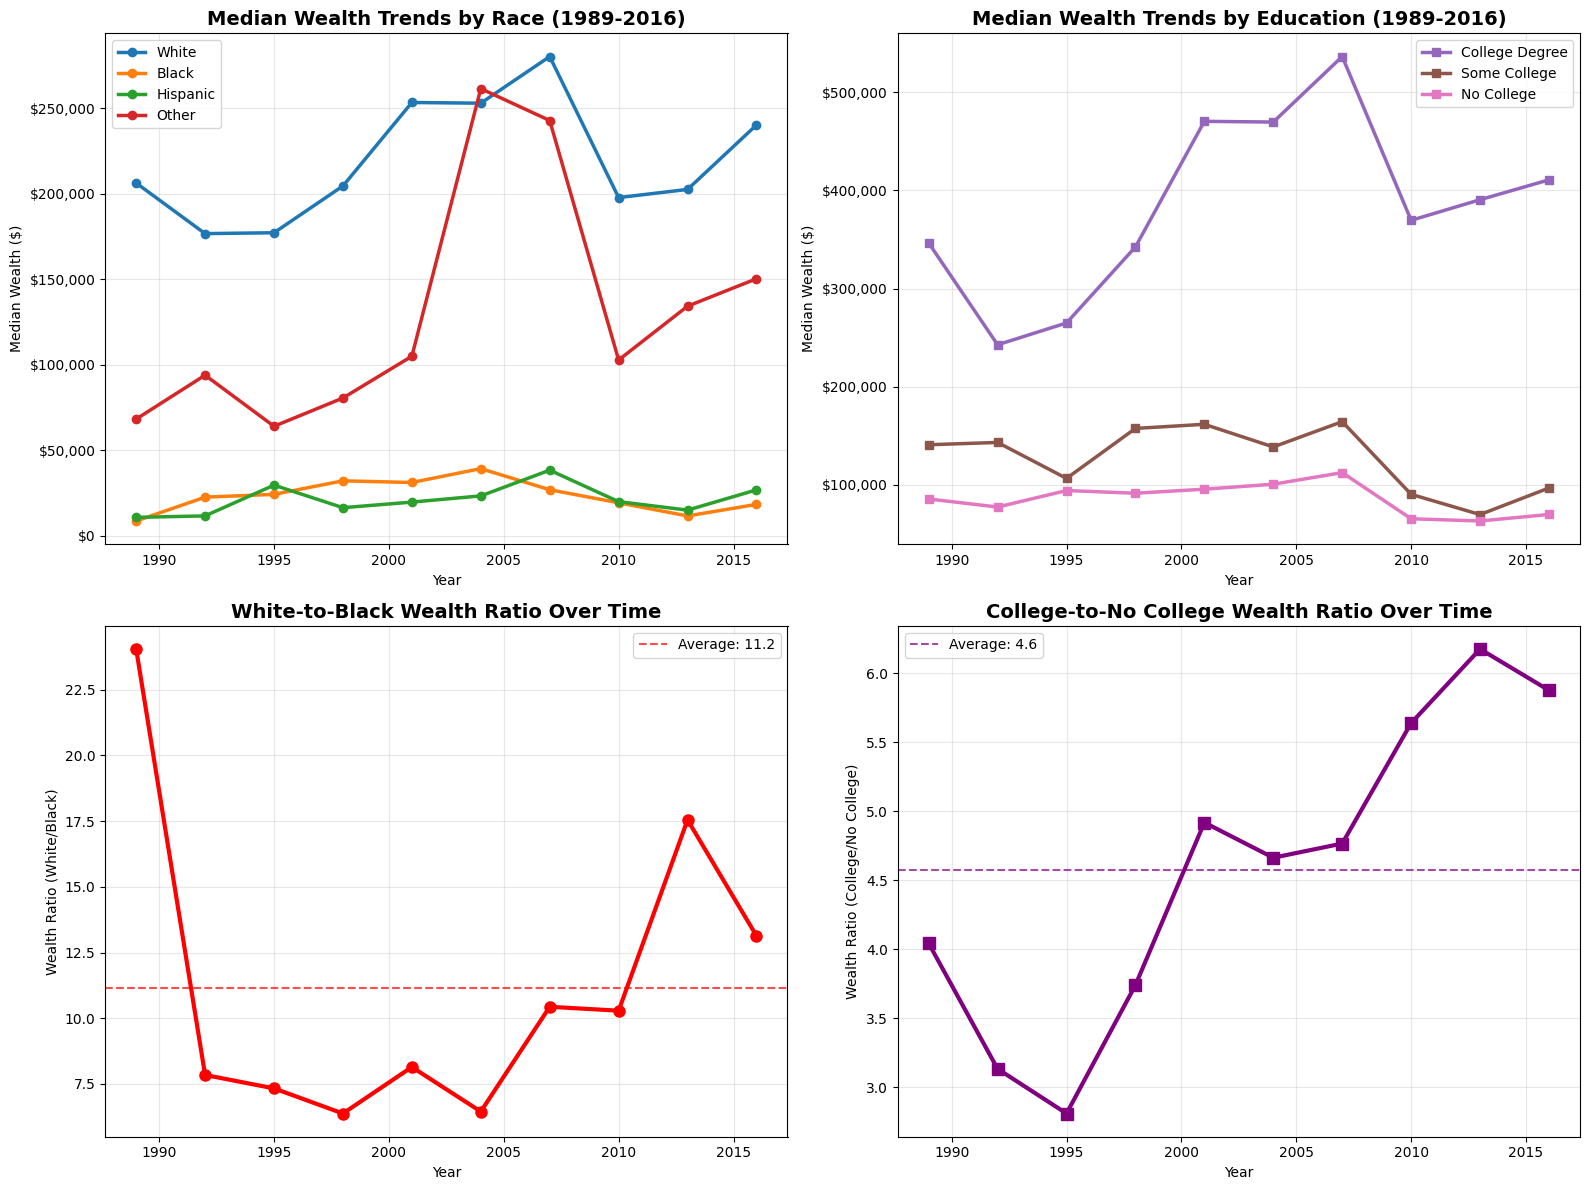
\includegraphics{Images/1.png} 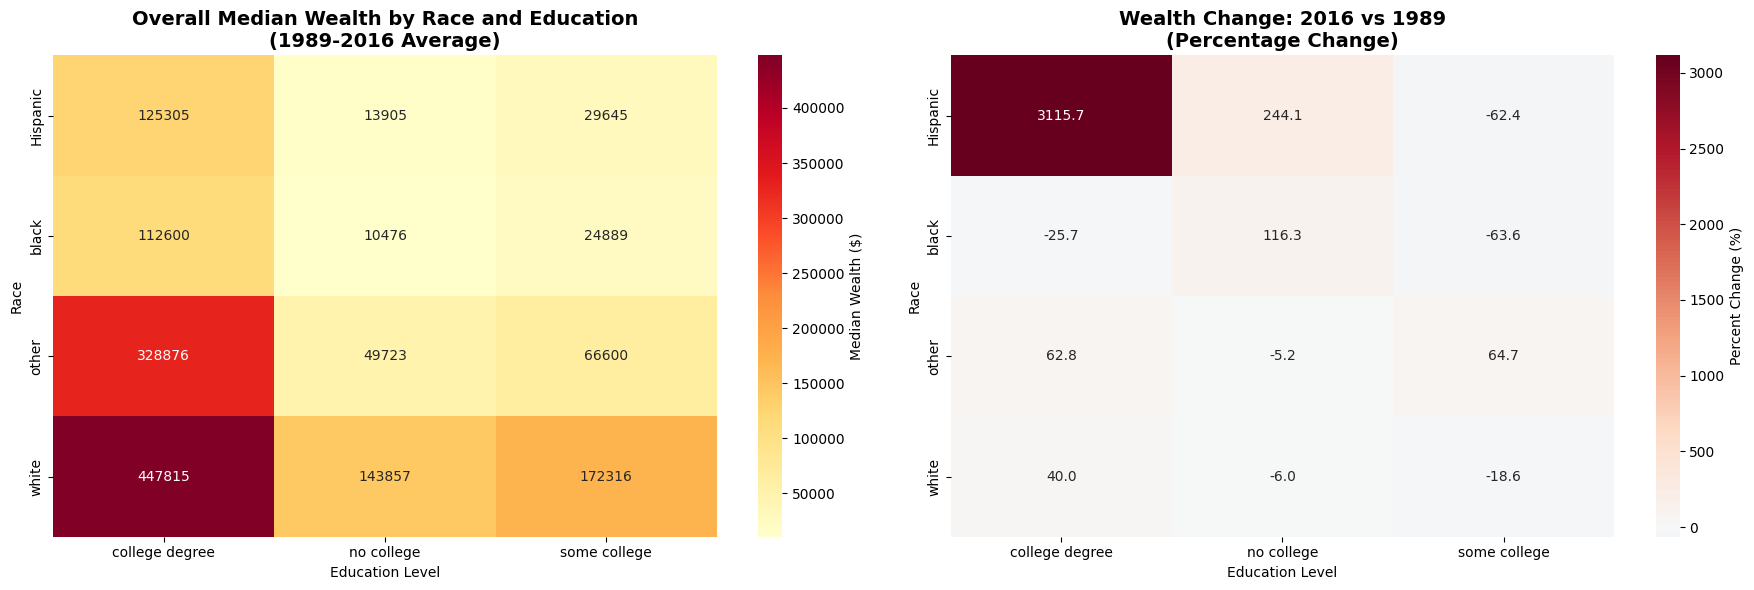
\includegraphics{Images/2.png}

\subsection{Race}\label{race}

\begin{itemize}
\tightlist
\item
  \textbf{White households} consistently maintain the highest median
  wealth
\item
  \textbf{Black households} have the lowest median wealth throughout
  most years
\item
  \textbf{Hispanic households} show similar patterns to Black
  households, with relatively higher wealth in recent years
\item
  \textbf{Other race households} show high volatility, with a dramatic
  spike in 2004--2007
\item
  The \textbf{White-to-Black wealth ratio} averages around 11x over the
  entire period
\item
  The gap was extreme in 1989 but narrowed considerably by the mid-1990s
\item
  The ratio has fluctuated throughout the sample period.
\end{itemize}

\subsection{Education}\label{education}

\begin{itemize}
\tightlist
\item
  \textbf{College degree holders} consistently have the highest median
  wealth.
\item
  \textbf{Some college} group falls in the middle.
\item
  \textbf{No college} group has the lowest wealth.
\item
  The \textbf{College-to-No College ratio} averages around 4.6
  throughout the sample period.
\item
  This gap has \textbf{widened significantly} over time.
\item
  The education premium peaked around 2010--2013.
\item
  The education gap shows a trend toward expansion.
\end{itemize}

\subsection{Comprehensive Wealth Analysis Summary
(1989--2016)}\label{comprehensive-wealth-analysis-summary-19892016}

\begin{longtable}[]{@{}
  >{\raggedright\arraybackslash}p{(\columnwidth - 12\tabcolsep) * \real{0.1429}}
  >{\raggedright\arraybackslash}p{(\columnwidth - 12\tabcolsep) * \real{0.1429}}
  >{\raggedright\arraybackslash}p{(\columnwidth - 12\tabcolsep) * \real{0.1429}}
  >{\raggedright\arraybackslash}p{(\columnwidth - 12\tabcolsep) * \real{0.1429}}
  >{\raggedright\arraybackslash}p{(\columnwidth - 12\tabcolsep) * \real{0.1429}}
  >{\raggedright\arraybackslash}p{(\columnwidth - 12\tabcolsep) * \real{0.1429}}
  >{\raggedright\arraybackslash}p{(\columnwidth - 12\tabcolsep) * \real{0.1429}}@{}}
\toprule\noalign{}
\begin{minipage}[b]{\linewidth}\raggedright
Metric
\end{minipage} & \begin{minipage}[b]{\linewidth}\raggedright
Group
\end{minipage} & \begin{minipage}[b]{\linewidth}\raggedright
1989 Value
\end{minipage} & \begin{minipage}[b]{\linewidth}\raggedright
2016 Value
\end{minipage} & \begin{minipage}[b]{\linewidth}\raggedright
\% Change (1989--2016)
\end{minipage} & \begin{minipage}[b]{\linewidth}\raggedright
CAGR
\end{minipage} & \begin{minipage}[b]{\linewidth}\raggedright
Notes
\end{minipage} \\
\midrule\noalign{}
\endhead
\bottomrule\noalign{}
\endlastfoot
\textbf{Median Wealth} & White & \$206,364 & \$240,350 & +16.5\% &
+0.57\% & Highest absolute wealth \\
& Black & \$8,583 & \$18,300 & +113.2\% & +2.84\% & Fastest growth
rate \\
& Hispanic & \$10,710 & \$26,800 & +150.2\% & +3.46\% & Largest \%
increase \\
& Other & \$68,234 & \$150,350 & +120.3\% & +2.97\% & High volatility
group \\
& College Degree & \$346,490 & \$410,800 & +18.6\% & +0.63\% & Highest
absolute wealth \\
& Some College & \$140,928 & \$96,905 & -31.2\% & -1.38\% & Significant
decline \\
& No College & \$85,699 & \$69,921 & -18.4\% & -0.75\% & Moderate
decline \\
\textbf{Wealth Gap Ratios} & White-to-Black & 24.0 & 13.1 & -45.4\% &
--- & Gap narrowed significantly \\
& College-to-No College & 4.0 & 5.9 & +45.3\% & --- & Gap widened
substantially \\
\textbf{Wealth Volatility (CV)} & White & --- & --- & --- & --- & 16.1\%
(lowest) \\
& Black & --- & --- & --- & --- & 40.4\% (high) \\
& Hispanic & --- & --- & --- & --- & 40.8\% (high) \\
& Other & --- & --- & --- & --- & 53.5\% (highest) \\
& College Degree & --- & --- & --- & --- & 23.9\% (moderate) \\
& Some College & --- & --- & --- & --- & 26.3\% (moderate) \\
& No College & --- & --- & --- & --- & 19.0\% (low) \\
\textbf{Financial Crisis Impact (2007-2010)} & White & --- & --- &
-29.4\% & --- & Moderate decline \\
& Black & --- & --- & -28.4\% & --- & Similar to White \\
& Hispanic & --- & --- & -48.1\% & --- & Severe impact \\
& Other & --- & --- & -57.7\% & --- & Most severe impact \\
& College Degree & --- & --- & -31.1\% & --- & Moderate decline \\
& Some College & --- & --- & -45.0\% & --- & Large decline \\
& No College & --- & --- & -41.8\% & --- & Significant decline \\
\end{longtable}

\section{Repeat your analysis for just median housing wealth for black
and white
households}\label{repeat-your-analysis-for-just-median-housing-wealth-for-black-and-white-households}

\begin{figure}[H]

{\centering 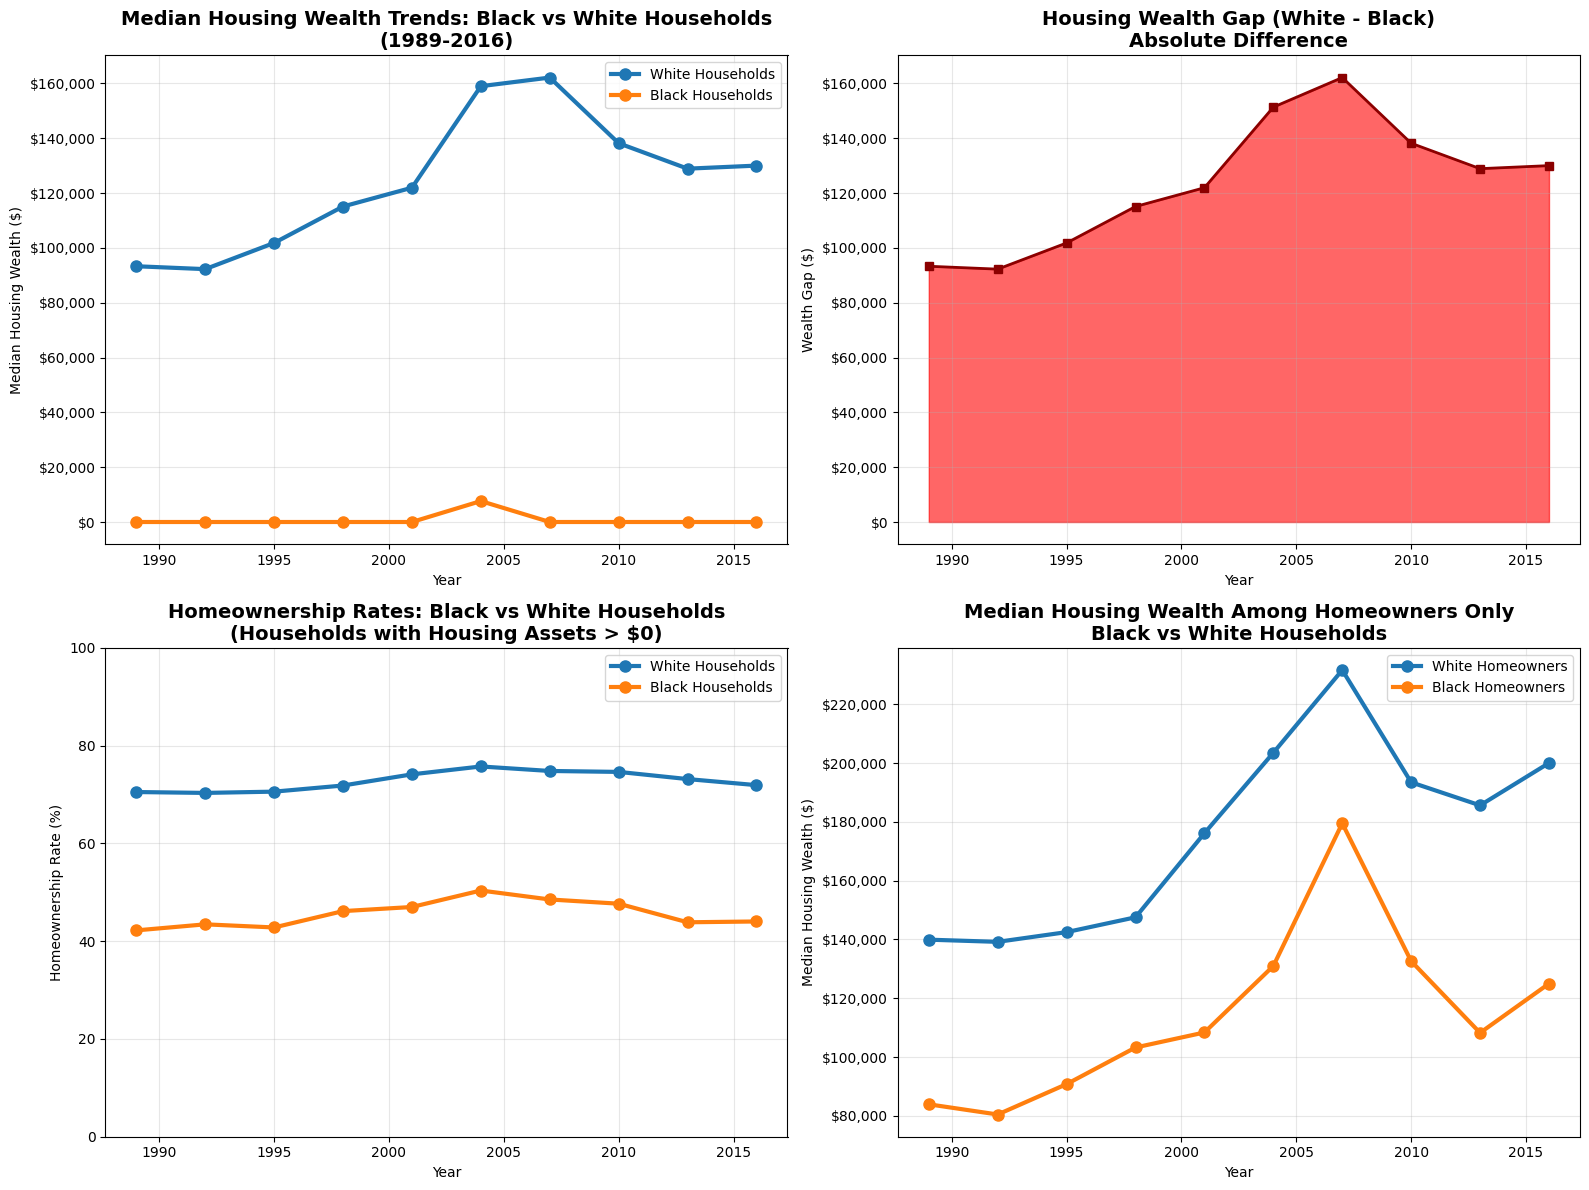
\includegraphics{Images/3.png}

}

\caption{Median Housing Wealth Black vs White}

\end{figure}%

\begin{longtable}[]{@{}
  >{\raggedright\arraybackslash}p{(\columnwidth - 12\tabcolsep) * \real{0.1250}}
  >{\raggedright\arraybackslash}p{(\columnwidth - 12\tabcolsep) * \real{0.1250}}
  >{\centering\arraybackslash}p{(\columnwidth - 12\tabcolsep) * \real{0.1562}}
  >{\centering\arraybackslash}p{(\columnwidth - 12\tabcolsep) * \real{0.1562}}
  >{\centering\arraybackslash}p{(\columnwidth - 12\tabcolsep) * \real{0.1562}}
  >{\centering\arraybackslash}p{(\columnwidth - 12\tabcolsep) * \real{0.1562}}
  >{\raggedright\arraybackslash}p{(\columnwidth - 12\tabcolsep) * \real{0.1250}}@{}}
\toprule\noalign{}
\begin{minipage}[b]{\linewidth}\raggedright
Metric
\end{minipage} & \begin{minipage}[b]{\linewidth}\raggedright
Group
\end{minipage} & \begin{minipage}[b]{\linewidth}\centering
1989
\end{minipage} & \begin{minipage}[b]{\linewidth}\centering
2016
\end{minipage} & \begin{minipage}[b]{\linewidth}\centering
\% Change
\end{minipage} & \begin{minipage}[b]{\linewidth}\centering
CAGR
\end{minipage} & \begin{minipage}[b]{\linewidth}\raggedright
Notes
\end{minipage} \\
\midrule\noalign{}
\endhead
\bottomrule\noalign{}
\endlastfoot
\textbf{Housing Wealth (All)} & White & \$93,293 & \$130,000 & +39.4\% &
+1.24\% & Substantial growth \\
& Black & \$0 & \$0 & 0\% & --- & Positive in 1/10 years \\
\textbf{Home ownership Rate} & White & 70.5\% & 71.9\% & +1.9\% & --- &
Avg: 72.8\% \\
& Black & 42.2\% & 44.0\% & +4.3\% & --- & Avg: 45.6\% \\
\textbf{Owner-ship Gap} & White-Black & 28.3 pp & 27.9 pp & -1.4\% & ---
& Avg: 27.2 pp \\
\textbf{Housing Wealth (Owners)} & White & \$139,940 & \$200,000 &
+42.9\% & --- & Among homeowners \\
& Black & \$83,964 & \$125,000 & +48.9\% & --- & Among homeowners \\
\textbf{Wealth Ratio (Owners)} & White/Black & 1.7 & 1.6 & -5.9\% & ---
& Gap narrowed \\
\textbf{Volatility (CV)} & White & --- & --- & --- & --- & 19.8\% \\
& Black & --- & --- & --- & --- & 25.7\% \\
\end{longtable}

\subsection{Findings}\label{findings}

\subsubsection{Stark housing wealth
divide}\label{stark-housing-wealth-divide}

\begin{itemize}
\tightlist
\item
  In 9 out of 10 survey years, more than half of Black households had
  zero median housing wealth.
\item
  White households maintained substantial median housing wealth
  (\$93K--\$162K) throughout.
\end{itemize}

\subsubsection{Persistent homeownership
gap}\label{persistent-homeownership-gap}

\begin{itemize}
\tightlist
\item
  White households: average homeownership rate 72.8\% (range:
  70.5\%--75.7\%)
\item
  Black households: average homeownership rate 45.6\% (range:
  42.2\%--50.4\%)
\item
  The homeownership gap (27.2 percentage points) has remained stable for
  nearly three decades.
\item
  This gap is a major barrier to wealth accumulation for Black families.
\end{itemize}

\subsubsection{Housing wealth among
homeowners}\label{housing-wealth-among-homeowners}

\begin{itemize}
\tightlist
\item
  Among homeowners, the racial gap narrows but persists.
\item
  In 1989, White homeowners had 1.7× the housing wealth of Black
  homeowners; in 2016, this ratio was 1.6×.
\item
  Both groups saw strong growth: +43\% for White homeowners, +49\% for
  Black homeowners.
\end{itemize}

\subsubsection{Growth patterns}\label{growth-patterns}

\begin{itemize}
\tightlist
\item
  White households experienced steady housing wealth growth (1.24\%
  annually), peaking during the 2004--2007 housing boom.
\item
  Black households showed a volatile pattern, with most years at zero
  median housing wealth.
\item
  The 2008 financial crisis affected both groups, but White households
  recovered more fully.
\end{itemize}

\subsubsection{Economic cycle impact}\label{economic-cycle-impact}

\begin{itemize}
\tightlist
\item
  During the 2001--2007 boom, both groups saw housing wealth increases.
\item
  The 2007--2010 crisis brought sharp declines for both groups.
\end{itemize}

\section{Many households are not homeowners and so your analysis for the
prior\ldots{}}\label{many-households-are-not-homeowners-and-so-your-analysis-for-the-prior}

\begin{figure}[H]

{\centering 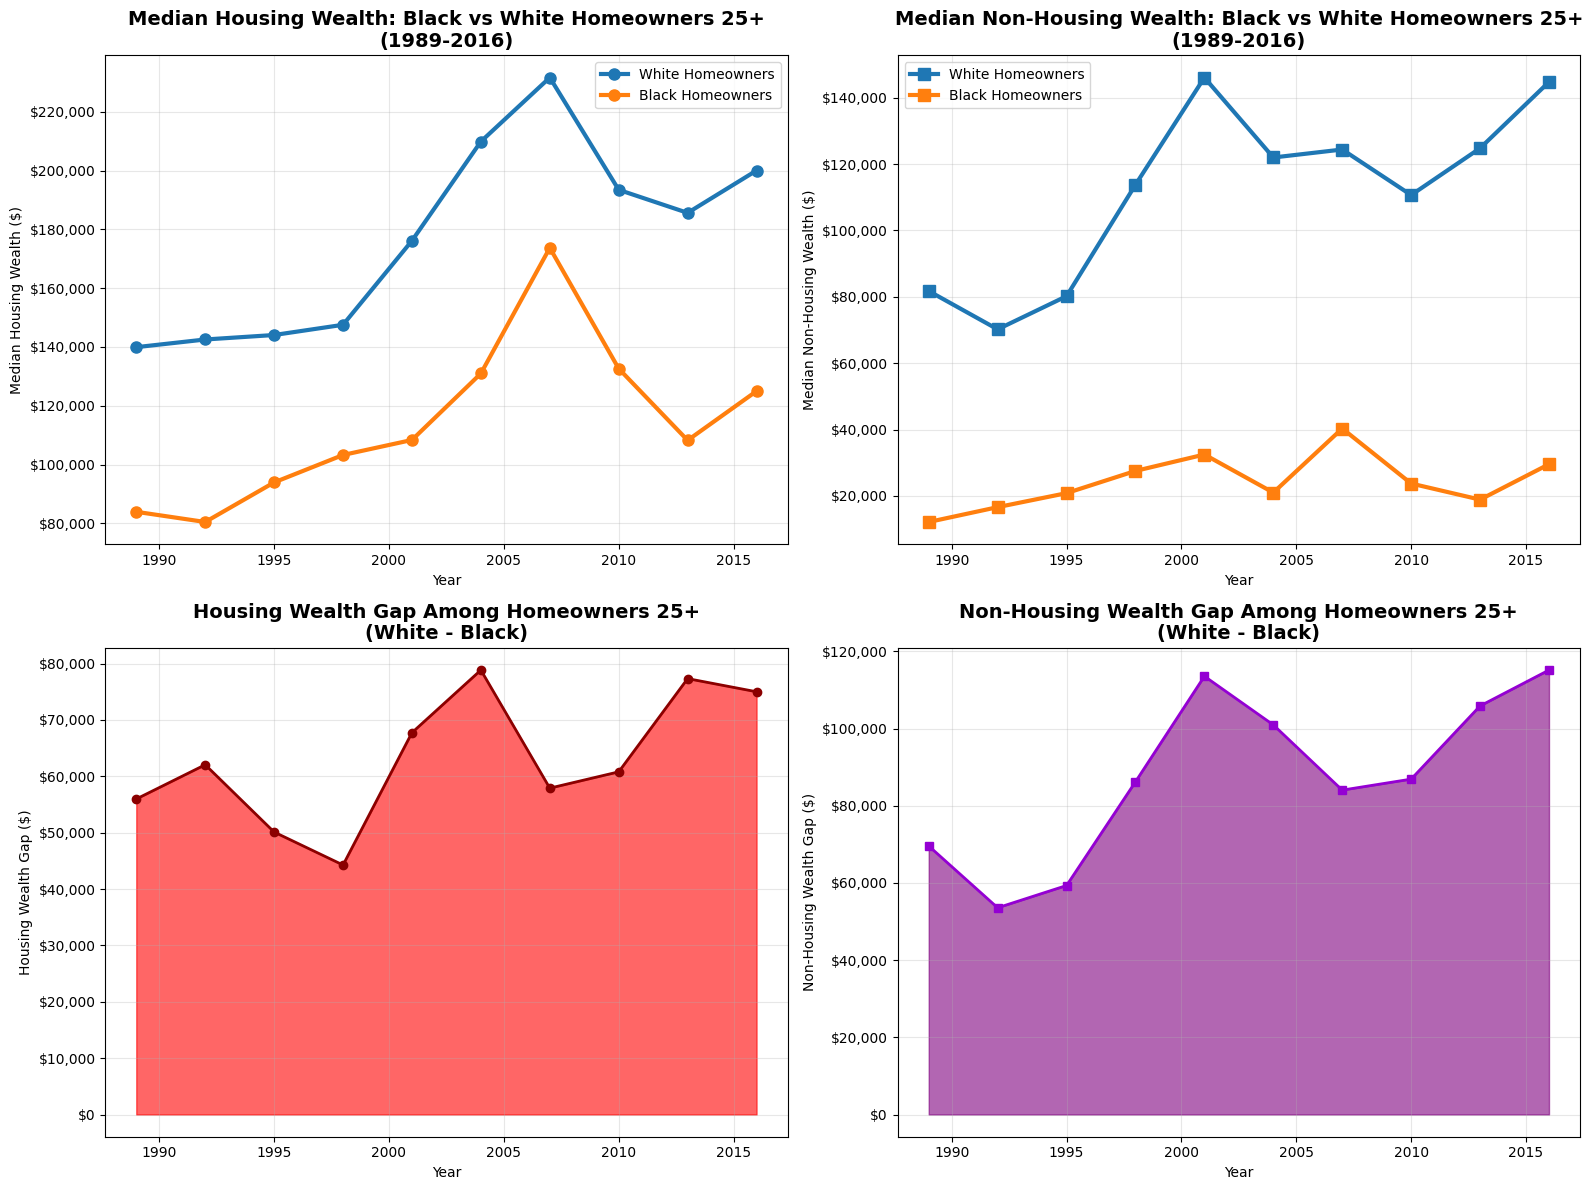
\includegraphics{Images/4.png}

}

\caption{Financial Crisis Impact Homeowners 25+}

\end{figure}%

\subsection{Homeowners Aged 25+ Analysis
Summary}\label{homeowners-aged-25-analysis-summary}

\textbf{Dataset:} 33,292 homeowners aged 25+ (69.7\% of total sample)\\
\textbf{Race Distribution:} White: 85.2\%, Black: 6.3\%, Hispanic:
4.7\%, Other: 3.7\%

\subsubsection{Median Housing Wealth by Year (Homeowners
25+)}\label{median-housing-wealth-by-year-homeowners-25}

\begin{longtable}[]{@{}cccc@{}}
\toprule\noalign{}
Year & Black & White & White/Black Ratio \\
\midrule\noalign{}
\endhead
\bottomrule\noalign{}
\endlastfoot
1989 & \$83,964 & \$139,940 & 1.7 \\
1992 & \$80,499 & \$142,551 & 1.8 \\
1995 & \$93,960 & \$144,072 & 1.5 \\
1998 & \$103,282 & \$147,546 & 1.4 \\
2001 & \$108,388 & \$176,131 & 1.6 \\
2004 & \$130,994 & \$209,844 & 1.6 \\
2007 & \$173,702 & \$231,603 & 1.3 \\
2010 & \$132,639 & \$193,433 & 1.5 \\
2013 & \$108,266 & \$185,599 & 1.7 \\
2016 & \$125,000 & \$200,000 & 1.6 \\
\end{longtable}

\subsubsection{Median Non-Housing Wealth by Year (Homeowners
25+)}\label{median-non-housing-wealth-by-year-homeowners-25}

\begin{longtable}[]{@{}cccc@{}}
\toprule\noalign{}
Year & Black & White & White/Black Ratio \\
\midrule\noalign{}
\endhead
\bottomrule\noalign{}
\endlastfoot
1989 & \$12,128 & \$81,725 & 6.7 \\
1992 & \$16,603 & \$70,185 & 4.2 \\
1995 & \$20,828 & \$80,179 & 3.8 \\
1998 & \$27,517 & \$113,758 & 4.1 \\
2001 & \$32,462 & \$146,053 & 4.5 \\
2004 & \$20,984 & \$121,964 & 5.8 \\
2007 & \$40,299 & \$124,371 & 3.1 \\
2010 & \$23,720 & \$110,643 & 4.7 \\
2013 & \$18,869 & \$124,764 & 6.6 \\
2016 & \$29,540 & \$144,730 & 4.9 \\
\end{longtable}

\subsubsection{Financial Crisis Impact and Recovery
Analysis}\label{financial-crisis-impact-and-recovery-analysis}

\begin{longtable}[]{@{}
  >{\raggedright\arraybackslash}p{(\columnwidth - 16\tabcolsep) * \real{0.0930}}
  >{\raggedright\arraybackslash}p{(\columnwidth - 16\tabcolsep) * \real{0.0930}}
  >{\centering\arraybackslash}p{(\columnwidth - 16\tabcolsep) * \real{0.1163}}
  >{\centering\arraybackslash}p{(\columnwidth - 16\tabcolsep) * \real{0.1163}}
  >{\centering\arraybackslash}p{(\columnwidth - 16\tabcolsep) * \real{0.1163}}
  >{\centering\arraybackslash}p{(\columnwidth - 16\tabcolsep) * \real{0.1163}}
  >{\centering\arraybackslash}p{(\columnwidth - 16\tabcolsep) * \real{0.1163}}
  >{\centering\arraybackslash}p{(\columnwidth - 16\tabcolsep) * \real{0.1163}}
  >{\centering\arraybackslash}p{(\columnwidth - 16\tabcolsep) * \real{0.1163}}@{}}
\toprule\noalign{}
\begin{minipage}[b]{\linewidth}\raggedright
Category
\end{minipage} & \begin{minipage}[b]{\linewidth}\raggedright
Group
\end{minipage} & \begin{minipage}[b]{\linewidth}\centering
2007 Peak
\end{minipage} & \begin{minipage}[b]{\linewidth}\centering
2010 Crisis
\end{minipage} & \begin{minipage}[b]{\linewidth}\centering
Dollar Change
\end{minipage} & \begin{minipage}[b]{\linewidth}\centering
\% Change
\end{minipage} & \begin{minipage}[b]{\linewidth}\centering
2016 Recovery
\end{minipage} & \begin{minipage}[b]{\linewidth}\centering
Recovery Rate
\end{minipage} & \begin{minipage}[b]{\linewidth}\centering
Volatility (CV)
\end{minipage} \\
\midrule\noalign{}
\endhead
\bottomrule\noalign{}
\endlastfoot
\textbf{Housing Wealth} & White & \$231,603 & \$193,433 & -\$38,170 &
-16.5\% & \$200,000 & 86.4\% (Partial) & 18.3\% \\
& Black & \$173,702 & \$132,639 & -\$41,063 & -23.6\% & \$125,000 &
72.0\% (Partial) & 24.3\% \\
\textbf{Non-Housing Wealth} & White & \$124,371 & \$110,643 & -\$13,727
& -11.0\% & \$144,730 & 116.4\% (Full) & 23.7\% \\
& Black & \$40,299 & \$23,720 & -\$16,579 & -41.1\% & \$29,540 & 73.3\%
(Partial) & 34.2\% \\
\end{longtable}

\subsubsection{Long-Term Growth and Composition Analysis
(1989-2016)}\label{long-term-growth-and-composition-analysis-1989-2016}

\begin{longtable}[]{@{}llll@{}}
\toprule\noalign{}
Metric & Group & Housing Wealth & Non-Housing Wealth \\
\midrule\noalign{}
\endhead
\bottomrule\noalign{}
\endlastfoot
\textbf{CAGR} & White & 1.33\% & 2.14\% \\
& Black & 1.48\% & 3.35\% \\
\textbf{Total Growth} & White & 42.9\% & 77.1\% \\
& Black & 48.9\% & 143.6\% \\
\textbf{1989 Composition} & White & 63.1\% housing & 36.9\%
non-housing \\
& Black & 87.4\% housing & 12.6\% non-housing \\
\textbf{2016 Composition} & White & 58.0\% housing & 42.0\%
non-housing \\
& Black & 80.9\% housing & 19.1\% non-housing \\
\end{longtable}

\subsubsection{Findings}\label{findings-1}

\paragraph{Median Housing Wealth:}\label{median-housing-wealth}

Both Black and White homeowners saw growth from 1989 to 2007, peaking in
2007.

\begin{itemize}
\tightlist
\item
  2007 Peak: White: \$231,603 \textbar{} Black: \$173,702
\item
  2010 Crisis: White: \$193,433 \textbar{} Black: \$132,639
\item
  2016 Recovery: White: \$200,000 \textbar{} Black: \$125,000
\end{itemize}

\paragraph{Median Non-Housing Wealth:}\label{median-non-housing-wealth}

Both groups saw non-housing wealth peak in 2007, decline in 2010, and
partial recovery by 2016.

\begin{itemize}
\tightlist
\item
  2007 Peak: White: \$124,371 \textbar{} Black: \$40,299
\item
  2010 Crisis: White: \$110,643 \textbar{} Black: \$23,720
\item
  2016 Recovery: White: \$144,730 \textbar{} Black: \$29,540
\end{itemize}

\paragraph{Loss in Housing Wealth
(2007)}\label{loss-in-housing-wealth-2007}

Dollar Terms:

\begin{itemize}
\tightlist
\item
  White: \$231,603 → \$193,433 = --\$38,170
\item
  Black: \$173,702 → \$132,639 = --\$41,063
\item
  Black homeowners had the largest dollar loss (\$41,063 vs.~\$38,170).
\end{itemize}

Proportional Terms (\% Loss):

\begin{itemize}
\tightlist
\item
  White: --16.5\%
\item
  Black: --23.6\%
\item
  Black homeowners also had the largest proportional loss.
\end{itemize}

\paragraph{Summary}\label{summary}

\begin{itemize}
\tightlist
\item
  Both Black and White homeowners aged 25+ experienced significant
  declines in housing wealth during the financial crisis (2007--2010).
\item
  Black homeowners had the largest loss in both dollar terms and
  proportional terms.
\item
  By 2016, neither group had fully recovered to 2007 levels, but White
  homeowners recovered a greater share of their losses.
\end{itemize}

\section{Many potential channels have been identified for explaining the
wealth}\label{many-potential-channels-have-been-identified-for-explaining-the-wealth}

\subsection{Hypothesis 1: Workplace Income
Discrimination}\label{hypothesis-1-workplace-income-discrimination}

One key mechanism by which discrimination widens racial wealth gaps is
through \textbf{income labor discrimination}. Persistent disparities in
income make it more difficult for Black households to accumulate assets
or manage debt as reliably as White households.

\subsubsection{Longitudinal Analysis of Income
Variation}\label{longitudinal-analysis-of-income-variation}

\begin{itemize}
\tightlist
\item
  Use longitudinal datasets such as the \emph{Panel Study of Income
  Dynamics (PSID)} to measure year-to-year income and income by race.
\item
  Estimate income outcome coefficients, controlling for education,
  occupation, experience, sex, and location.
\item
  This approach isolates the contribution of discrimination to income
  differences, above and beyond observable characteristics.
\end{itemize}

\subsubsection{Event Study Strategy}\label{event-study-strategy}

\begin{itemize}
\tightlist
\item
  Compare firms, industries, or states with \textbf{inclusionary
  policies} (e.g., diversity initiatives, pay transparency laws) to
  those with \textbf{exclusionary practices} (e.g., documented
  discrimination cases).
\item
  Include a \textbf{neutral group} of firms or states as a control.
\item
  Estimate effects on income controlling for race. A triple-difference
  specification,
  \[(\text{Inclusionary} - \text{Exclusionary} - \text{Control}),\]
  provides stronger identification, while a simpler difference
  (Exclusionary vs.~Non-exclusionary) serves as a robustness check.
\end{itemize}

\subsubsection{Expected Contribution}\label{expected-contribution}

By focusing on income \(β\) coefficient across different policy
environments, this approach highlights how workplace discrimination
affects income. The key test is whether inclusive versus exclusionary
environments produce systematically different income patterns across
racial groups.

\subsection{Hypothesis 2: Disparities in the Transmission of Investment
Knowledge}\label{hypothesis-2-disparities-in-the-transmission-of-investment-knowledge}

Another important mechanism sustaining the racial wealth gap is
\textbf{unequal transmission of investment knowledge}. Even among
households with similar incomes and access to financial products, Black
parents may be less likely to transmit financial knowledge---such as
saving habits or familiarity with financial instruments like
401(k)s---to their children. These differences in financial literacy and
exposure to sound financial advice can generate divergent wealth
trajectories.

\subsubsection{Intergenerational Transmission of Financial
Knowledge}\label{intergenerational-transmission-of-financial-knowledge}

\begin{itemize}
\tightlist
\item
  Construct a dataset linking parents and children (e.g., using the PSID
  or other intergenerational surveys).
\item
  Use indicators of parental financial sophistication (e.g., whether
  parents have a 401(k), stock holdings, or savings rate).
\item
  Test whether parental financial sophistication predicts children's
  financial sophistication.
\item
  Estimate a triple-difference specification: \begin{align*}
    & \Big( \text{Black w/ financially active parents} \\
    & \quad - \text{Black w/o financially active parents} \Big) \\
    & - \Big( \text{White w/ financially active parents} \\
    & \quad - \text{White w/o financially active parents} \Big)
  \end{align*}
\item
  This identifies whether financial knowledge is transmitted differently
  across racial groups, which could be a driving force behind the wealth
  gap.
\item
  Additionally, examine whether the savings rate of parents is similarly
  transmitted to children, controlling for race.
\end{itemize}

\subsubsection{Neighborhood Transmission of Financial
Knowledge}\label{neighborhood-transmission-of-financial-knowledge}

This analysis can be extended to the neighborhood level. Children may
acquire financial knowledge not only from parents but also through
neighborhood connections. - Measure neighborhood financial
sophistication (e.g., share of households with retirement accounts,
stock ownership, or savings rate). - Test whether Black individuals in
financially sophisticated neighborhoods experience high levels of
financial sophistication. This may be an important observation, given
that white-majority, financially sophisticated neighborhoods may not
necessarily transmit financial sophistication to minority Black members
of the neighborhood. - Compare whether these neighborhood effects
operate equally for Black and White households, using the same
triple-difference estimator as above.

\subsubsection{Expected Contribution}\label{expected-contribution-1}

By separately identifying family-based and neighborhood-based channels,
and testing whether these operate differently by race, we can assess how
much of the wealth gap is driven by \textbf{differences in transmission
of financial knowledge} that affect asset holdings.

\subsection{Assessing the Importance of Each
Channel}\label{assessing-the-importance-of-each-channel}

To evaluate the importance of these channels, we can extract the
coefficients from our income labor discrimination estimates. This would
give us a dollar amount that we can use to evaluate the magnitude of our
estimates and their relation to overall wealth. These coefficients would
also be helpful in comparing against other estimates academics have
produced.

Next, with regard to the financial sophistication transmission channel,
we can use these estimates to obtain coefficients that measure the
financial sophistication associated with neighbor or family
transmission. To assess the importance of these, we would create an
additional test examining whether individuals with greater financial
sophistication tend to have higher asset holdings. This can be done
using a simple regression, controlling for age, race, gender, etc., with
financial sophistication as the independent variable and assets as the
dependent variable. The coefficient from this regression would identify
asset increases associated with higher financial sophistication. This
provides a dollar estimate to assess the magnitude and importance of
financial literacy, and thus the significance of the financial
sophistication transmission channel. Furthermore, this is a well-studied
area, so other academic papers can be referenced to benchmark the
magnitude and importance of financial sophistication for asset
accumulation.

Finally, we can compare our estimates to findings from other academic
studies, while also checking for statistical significance and
robustness.



\end{document}
